\documentclass[10pt,letterpaper]{article}
\usepackage[dvipsnames]{xcolor}
\usepackage{outlines}
\usepackage{amsmath}
\usepackage{tikz}
\usepackage{hyperref}
\usepackage{enumitem}
\usepackage{cancel}
\usepackage{subcaption}
\DeclareCaptionOptionNoValue{centering}{\centering} % Make sure everything is centered in subs
\captionsetup[sub]{centering}

\usepackage{algorithm}
\usepackage[noend]{algpseudocode}
\makeatletter
\def\BState{\State\hskip-\ALG@thistlm}
\makeatother

\usepackage{multirow}
\usepackage{cancel}
\usepackage{float}

\usepackage{parskip}

\usepackage{slantsc,lmodern}

\usepackage{pgfplotstable,booktabs}
\usepackage{framed}
\definecolor{shadecolor}{rgb}{0.9,0.9,0.9}

\usepackage{gensymb}

\usepackage{paralist}

\usepackage[paper=a4paper,margin=1in]{geometry}

\usepackage{etoolbox}

\newcommand{\volume}{{\ooalign{\hfil$V$\hfil\cr\kern0.08em--\hfil\cr}}}

\makeatletter
\g@addto@macro\@floatboxreset\centering
\makeatother

\author{Thaddeus Hughes \\ hughes.thad@gmail.com \\ thaddeus-maximus.github.io}
\date{\today}
\title{Transient Modeling of Flywheel-Based Pitchers}



\begin{document}
	\maketitle
	
	\begin{abstract}
		Flywheel based pitchers are very common ways to propel projectiles. They are well-suited to many such cases in that they are reasonably light, do not require keeping track of states, provide inherent strength-of-shot adjustment, and can be used in continous applications.

		Unfortunately, they are somewhat of a mystery, with design essentially relegated to trial-and-error rather than intuitive understanding or numerical simulation. This paper aims to change that.
	\end{abstract}
	\newpage
	
	\section*{Hooded Pitcher}
	
	Consider the following \textit{hooded} pitcher. A wheel (red) is spun up to an initial RPM, and then a ball (blue) is introduced between it and an arced hood (black), which is concentric with the wheel.

	\begin{figure}[H]
	\includegraphics[height=2.5in]{hood_pitcher.jpeg}
	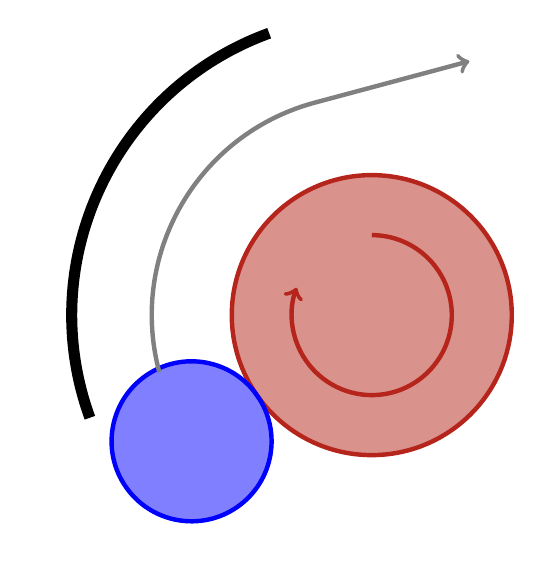
\begin{tikzpicture}[x=1in, y=1in]
	\fill[BrickRed, ultra thick, opacity=0.5] (0,0) circle(0.7);
	\draw[BrickRed,  ultra thick] (0,0) circle (0.7);
	\draw[BrickRed, ultra thick, ->] (0,0.4) arc(90:-200:0.4);
	\draw[black, ultra thick, rotate=20, line width=4] (-1.5,0) arc (180:90:1.5);
	\fill[Blue, ultra thick, rotate=35, opacity=0.5] (-1.1,0) circle(0.4);
	\draw[Blue, ultra thick, rotate=35] (-1.1,0) circle(0.4);
	\draw[gray, ultra thick, rotate=15, ->] (-1.1,0) arc (180:90:1.1) -- (0.8,1.1);
	\end{tikzpicture}
	\caption{Hooded pitcher: example and schematic.}
	\end{figure}

	% [d_b, m_b, moi_rat_b, k_b, w, d_w, I_w, mu_w, mu_h, omega_w_0, theta_0, theta_end] = params_pack;

	There are already many parameters of interest in this system.
	\begin{asparaenum}[]
		\item \textbf{$d_w$}, the wheel diameter
		\item $I_w$, the wheel's moment of inertia
		\item $\omega_{w,0}$, the wheel's initial velocity
		\item $d_b$, the ball's initial diameter
		\item $I_b$, the ball's moment of inertia
		\item $w$, the gap between the hood and the surface of the wheel
		\item $\theta$, the angle between inlet and outlet
	\end{asparaenum}

	What makes this work? The ball is accelerated as the wheel makes contact with the ball. The hood provides constraint, keeping the ball from simply spinning. Free-body diagrams may make this more clear.

	\begin{figure}[H]
	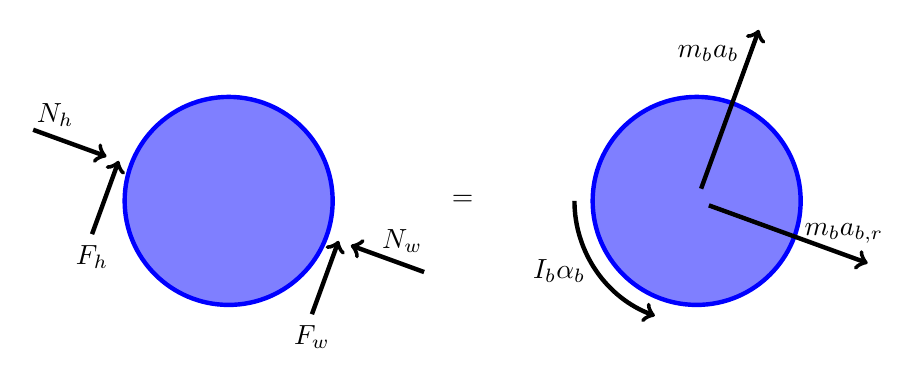
\begin{tikzpicture}[x=1.3in, y=1.3in]
	\fill[Blue, ultra thick, opacity=0.5] (0,0) circle(0.4);
	\draw[Blue, ultra thick] (0,0) circle(0.4);
	\draw[Black, ultra thick, ->, rotate=-20] (.8,0) -- (0.5,0) node[pos=0.3, above]{$N_w$};
	\draw[Black, ultra thick, ->, rotate=-20] (-.8,0) -- (-0.5,0) node[pos=0.3, above]{$N_h$};
	\draw[Black, ultra thick, ->, rotate=-20] (0.45,-0.3) -- (0.45,0) node[pos=0, below]{$F_w$};
	\draw[Black, ultra thick, ->, rotate=-20] (-0.45,-0.3) -- (-0.45,0) node[pos=0, below]{$F_h$};

	\node[black] at (0.9,0) {=} ;

	\fill[Blue, ultra thick, opacity=0.5] (1.8,0) circle(0.4);
	\draw[Blue, ultra thick] (1.8,0) circle(0.4);

	\draw[Black, ultra thick, ->, shift={(1.8,0)}, rotate=-20] (0,0.05) -- (0,0.7) node[pos=0.85, left]{$m_b a_b$};
	\draw[Black, ultra thick, ->, shift={(1.8,0)}, rotate=-20] (0.05,0) -- (0.7,0) node[pos=0.85, above]{$m_b a_{b,r}$};
	\draw[Black, ultra thick, ->, shift={(1.8,0)}] (-0.47,0) arc (180:250:0.47) node[pos=0.5, left]{$I_b \alpha_b$};
	\end{tikzpicture}
	\caption{Free-Body and Kinetic Diagrams for Ball}
	\end{figure}

	For the sake of simplicity, gravity is neglected during this split-second interaction. This leads to force balances

	\begin{align}
		F_h + F_w = m_b a_b \\
		N_h - N_w = m_b a_{b,r} = m_b \frac{v_b^2}{R}\\
		(F_w - F_h) \frac{w}{2} = I_b \alpha_b ,
	\end{align}

	where $R$ is the radius of the path travelled by the ball ($R = \frac{d_w + w}{2}$).

	\begin{figure}[H]
	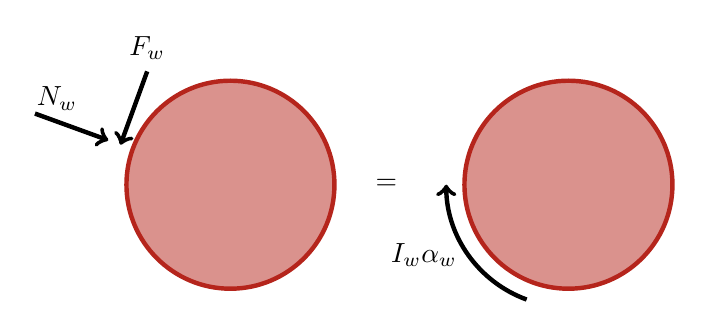
\begin{tikzpicture}[x=1.3in, y=1.3in]
	\fill[BrickRed, ultra thick, opacity=0.5] (0,0) circle(0.4);
	\draw[BrickRed, ultra thick] (0,0) circle(0.4);
	\draw[Black, ultra thick, ->, rotate=-20] (-.8,0) -- (-0.5,0) node[pos=0.3, above]{$N_w$};
	\draw[Black, ultra thick, ->, rotate=-20] (-0.45,0.3) -- (-0.45,0) node[pos=0, above]{$F_w$};

	\node[black] at (0.6,0) {=} ;

	\fill[BrickRed, ultra thick, opacity=0.5] (1.3,0) circle(0.4);
	\draw[BrickRed, ultra thick] (1.3,0) circle(0.4);
	\draw[Black, ultra thick, <-, shift={(1.3,0)}] (-0.47,0) arc (180:250:0.47) node[pos=0.5, left]{$I_w \alpha_w$};
	\end{tikzpicture}
	\caption{Free-Body and Kinetic Diagrams for Wheel}
	\end{figure}

	This leads to the torque balance

	\begin{align}
		- N_w \frac{d_w}{2} = I_w \alpha_w
	\end{align}

	At this point we have four governing equations, four unknown forces, and four unknown kinematic properties. Let's recap and solve what we have so far to get expressions for the accelerations.

	\begin{align}
		\alpha_{b}	&= (F_w - F_h) \frac{w}{2 I_b} \\
		a_b 		&= \frac{F_h + F_w}{m_b} \\
		\alpha_{w}	&= - F_w \frac{d_w}{2 I_w}
	\end{align}

	Where does the normal force come from? Well, it comes from the ball's compression! But the ball is also accelerating along the axis of the compression, making this not quite straightforward.

	\begin{figure}[H]
	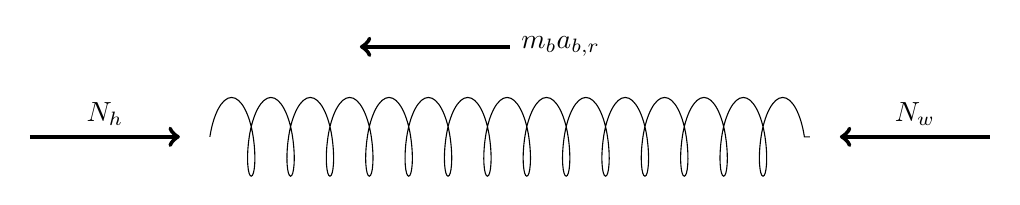
\begin{tikzpicture}[x=1.5in, y=1.5in]
		\draw[decoration={aspect=0.3, segment length=5mm, amplitude=5mm,coil},decorate] (-1,0) -- (+1,0);
		\draw[->, ultra thick] (-1.6,0) -- (-1.1,0) node[pos=0.5, above]{$N_h$};
		\draw[->, ultra thick] (+1.6,0) -- (+1.1,0) node[pos=0.5, above]{$N_w$};
		\draw[->, ultra thick] (0,0.3) -- (-0.5,0.3) node[pos=0, right]{$m_b a_{b,r}$};
	\end{tikzpicture}
	\caption{Massed spring model of the ball.}
	\end{figure}

	The inertial forces can be resolved in such a spring of stiffness $k_b$ squeezed by $\delta$ as so:
	\begin{align}
		N_h = k_b \delta + \frac{m_b a_{b,r}}{2} = k_b \delta + \frac{m_b v_b^2}{2 R} \\
		N_w = k_b \delta - \frac{m_b a_{b,r}}{2} = k_b \delta - \frac{m_b v_b^2}{2 R}
	\end{align}

	\textit{Side takeaway: As the ball accelerates through the hood, it lifts off the wheel. This effect is magnified with a smaller arc radius.}

	We can relate the normal forces to the frictional or tangential forces with a basic coloumb friction model. More sophisticated models are probably more accurate, but the intent of this model is to provide intuitively understandable results and general guidelines which should be followed up by real-world testing, so this is an appropriate model.

	\begin{align}
		F_h \leq \mu_h N_h \ & sign(0 - v_{b,top}) \\
		F_w \leq \mu_w N_w \ & sign(v_{w,surf} - v_{b,bottom})
	\end{align}

	Anyone who's simulated anything can immediately see the glaring problem here- sign functions have glaring discontinuities. There are many strategies to solve this. Here's what I've come up with.

	First, recognize that the sign associated with the wheel should either be positive or zero. The ball isn't going to start over-spinning with the wheel.
	Second, recognize that the spin of the ball should never exceed the speed of the ball such that the top of the ball travels backwards, so its sign should be negative or zero.
	Third, the sign becomes zero, the condition to calculate is no longer one of two surfaces at arbitrary velocities exchanging forces, but of two surfaces that have \textit{coupled}. This brings the driving physics away from force balance and towards pure kinematics. That is to say,

	\begin{align}
		v_{w,surf} = v_{b,bottom} \nonumber \\
		a_{w,surf} = a_{b,bottom} \nonumber \\
		\alpha_{w} \frac{d_w}{2} = a_{b} + \alpha_{b} \frac{w}{2}
	\end{align}

	and

	\begin{align}
		0 = v_{b,top} \nonumber \\
		0 = a_{b,top} \nonumber \\
		0 = a_{b} - \alpha_{b} \frac{w}{2} .
	\end{align}

	Substituting what we found earlier about the accelerations gives us

	\begin{align}
		- F_w \frac{d_w}{2 I_w} \frac{d_w}{2} = \frac{F_h + F_w}{m_b} + (F_w - F_h) \frac{w}{2 I_b} \frac{w}{2} \nonumber \\
		F_w \frac{d_w}{2 I_w} + \frac{F_w}{m_b} + F_w \frac{w}{2 I_b} \frac{w}{2} = - \frac{F_h}{m_b} + F_h \frac{w}{2 I_b} \frac{w}{2} \nonumber \\
		F_w = F_h \frac{\frac{w^2}{4 I_b} - \frac{1}{m_b}}{\frac{d_w}{2 I_w} + \frac{1}{m_b} + \frac{w^2}{4 I_b}}
	\end{align}

	in the case of no wheel slip, and

	\begin{align}
		0 = \frac{F_h + F_w}{m_b} - (F_w - F_h) \frac{w}{2 I_b} \frac{w}{2} \nonumber \\
		\frac{F_h}{m_b} + F_h \frac{w}{2 I_b} \frac{w}{2} = - \frac{F_w}{m_b} + F_h \frac{w}{2 I_b} \frac{w}{2} \nonumber \\
		F_h = F_w \frac{\frac{w^2}{4 I_b} - \frac{1}{m_b}}{\frac{w^2}{4 I_b} + \frac{1}{m_b}} 
	\end{align}

	in the case of no hood slip. In these cases, the force of one is directly proportional to the other. This means that when both hood and wheel stop slipping,

	\begin{align}
		F_h = F_w = 0
	\end{align}

	But how is state determined? We simply go back to the sign equations.
	\begin{align}
		\textit{top attached when } 0 \leq v_{b} - \omega_{b} \frac{w}{2} \\
		\textit{bottom attached when } \omega_{w} \frac{d_w}{2} \leq v_{b} + \omega_{b} \frac{w}{2}
	\end{align}

	This developed friction model can be summarized with this pseudocode, which would be ran every iteration of the simulation loop.

\begin{algorithm}
	\begin{algorithmic}
	\State $\textit{Fw} \gets \textit{mw Nw}$
	\State $\textit{Fh} \gets \textit{mh Nh}$
	\If{$\textit{hood attached} \ \text{and} \ \textit{wheel attached}$}
	\State $\textit{Fw} \gets 0$
	\State $\textit{Fh} \gets 0$
	\ElsIf{$\textit{wheel attached}$}
	\State $\textit{Fw} \gets \textit{Fw in attached state}$
	\ElsIf{$\textit{hood attached}$}
	\State $\textit{Fh} \gets \textit{Fh in attached state}$
	\EndIf
	\BState
	\BState $\textit{... insert interesting simulation code ...}$
	\BState
	\If{$\textit{ball top speed goes positive}$}
	\State $\textit{hood attached} \gets \text{true}$
	\EndIf
	\If{$\textit{ball bottom speed exceeds wheel speed}$}
	\State $\textit{wheel attached} \gets \text{true}$
	\EndIf
	\end{algorithmic}
\end{algorithm}

	All that's left is to set up the state equations and initial conditions.

	\begin{align}
		\frac{d}{dt} \omega_b &= \alpha_b \\
		\frac{d}{dt} v_b &= a_b \\
		\frac{d}{dt} u_b &= v_b \\
		\frac{d}{dt} \omega_w &= \alpha_w \\
		v_b(0) &= 0 \\
		u_b(0) &= 0 \\
		\omega_w(0) &= \omega_{w,0} \\
		\textit{when} \ u_b &\geq \theta R \ \textit{terminate}
	\end{align}

\section*{Dual-Wheel Pitchers}

Dual wheel pitchers are a little more complex as the effective gap is not constant during the ball's motion, and the wheel's normal forces contribute to ball acceleration. However, the basic strategy remains the same.

\begin{figure}[H]
	\includegraphics[height=2.5in]{dual_pitcher.png}
	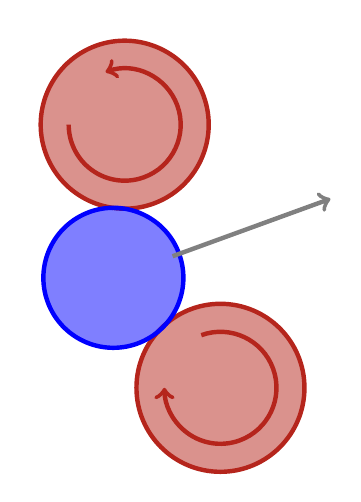
\begin{tikzpicture}[x=0.7in, y=0.7in]
	\fill[BrickRed, ultra thick, opacity=0.5] (0,0) circle(0.6);
	\draw[BrickRed,  ultra thick] (0,0) circle (0.6);
	\fill[BrickRed, ultra thick, opacity=0.5, rotate=20] (0,2) circle(0.6);
	\draw[BrickRed,  ultra thick, rotate=20] (0,2) circle (0.6);
	\draw[BrickRed, ultra thick, ->, rotate=20] (0,0.4) arc(90:-200:0.4);
	\draw[BrickRed, ultra thick, <-, rotate=20] (0,2.4) arc(90:-200:0.4);
	\fill[Blue, ultra thick, rotate=20, opacity=0.5] (-0.45,1) circle(0.5);
	\draw[Blue, ultra thick, rotate=20] (-0.45,1) circle(0.5);
	\draw[gray, ultra thick, rotate=20, ->] (0,1) -- (1.2,1);
	\end{tikzpicture}
	\caption{Dual wheel pitcher: example and schematic.}
\end{figure}

Some critical dimensions are:

\begin{figure}[H]
	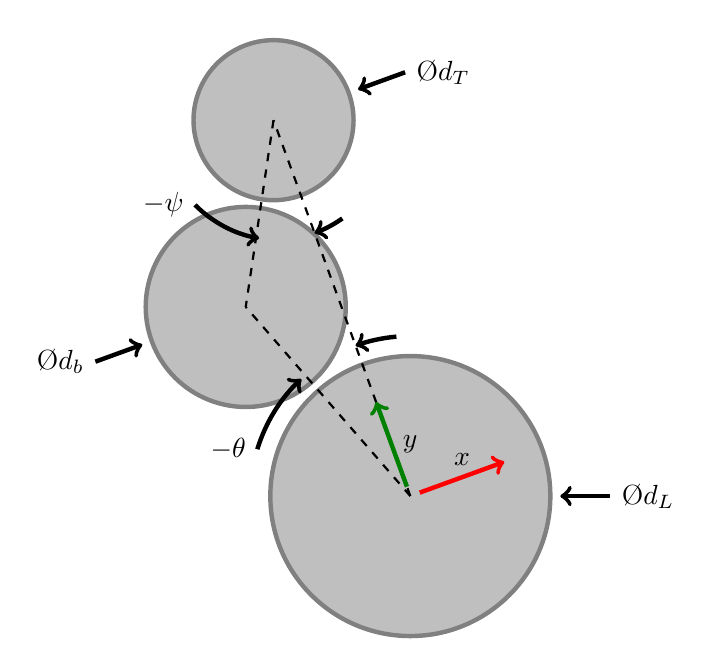
\begin{tikzpicture}[x=1in, y=1in]
	\fill[gray, ultra thick, opacity=0.5] (0,0) circle(0.7);
	\draw[gray,  ultra thick] (0,0) circle (0.7);
	\fill[gray, ultra thick, opacity=0.5, rotate=20] (0,2) circle(0.4);
	\draw[gray,  ultra thick, rotate=20] (0,2) circle (0.4);
	\fill[gray, ultra thick, rotate=20, opacity=0.5] (-0.45,1.17) circle(0.5);
	\draw[gray, ultra thick, rotate=20] (-0.45,1.17) circle(0.5);
	\draw[black, dashed, thick, rotate=20] (0,0) -- (0,2);
	\draw[black, dashed, thick, rotate=20] (0,0) -- (-0.45,1.17);
	\draw[black, dashed, thick, rotate=20] (0,2) -- (-0.45,1.17);
	\draw[black, ultra thick, <-] (0.75,0) -- (1.0,0) node[pos=1,right]{Ø$d_L$};
	\draw[black, ultra thick, <-, rotate=20] (0.45,2) -- (0.7,2) node[pos=1,right]{Ø$d_T$};
	\draw[black, ultra thick, <-, rotate=20] (-1.0,1.17) -- (-1.25,1.17) node[pos=1,left]{Ø$d_b$};
	\draw[red, ultra thick, ->, rotate=20] (0.05,0) -- (0.5,0) node[black,pos=0.5,above]{$x$};
	\draw[Green, ultra thick, ->, rotate=20] (0,0.05) -- (0,0.5) node[black,pos=0.5,right]{$y$};
	\draw[black, ultra thick, <-, rotate=20] (0,0.8) arc(90:75:0.8);
	\draw[black, ultra thick, <-, rotate=43] (0,0.8) arc(90:120:0.8) node[pos=1,left]{$- \theta$};
	\draw[black, ultra thick, <-, rotate=20] (0,1.4) arc(270:285:0.6);
	\draw[black, ultra thick, <-, rotate=20] (-0.27,1.47) arc(240:205:0.6) node[pos=1,left]{$- \psi$};
	\end{tikzpicture}
	\caption{Dual wheel pitcher key dimensions and coordinates. Note sign on angles.}
\end{figure}

Geometry allows us to relate these as so:
\begin{align}
	tan \theta &= \frac{x}{y} \\
	tan \psi   &= \frac{x}{\frac{d_L+d_T}{2} + w - y}
\end{align}

%Note at the beginning (and end),
%\begin{align}
%	x &= \frac{d_b + d_L}{2} sin \theta \\
%	x &= \frac{d_b + d_T}{2} sin \psi \\
%	y &= \frac{d_b + d_L}{2} cos \theta \\
%	y &= \frac{d_L+d_T}{2} + w - \frac{d_b + d_T}{2} cos \psi
%\end{align}

The instantaneous radii of the ball (distance from center of ball to top and bottom wheels) can be readily computed.
\begin{align}
	R_B = \sqrt{x^2 + y^2} - \frac{d_B}{2} \\
	R_T = \sqrt{x^2 + (\frac{d_T+d_B}{2} + w - y)^2} - \frac{d_T}{2}
\end{align}

To analyze the ball, begin by drawing free-body and kinetic diagrams.

\begin{figure}[H]
	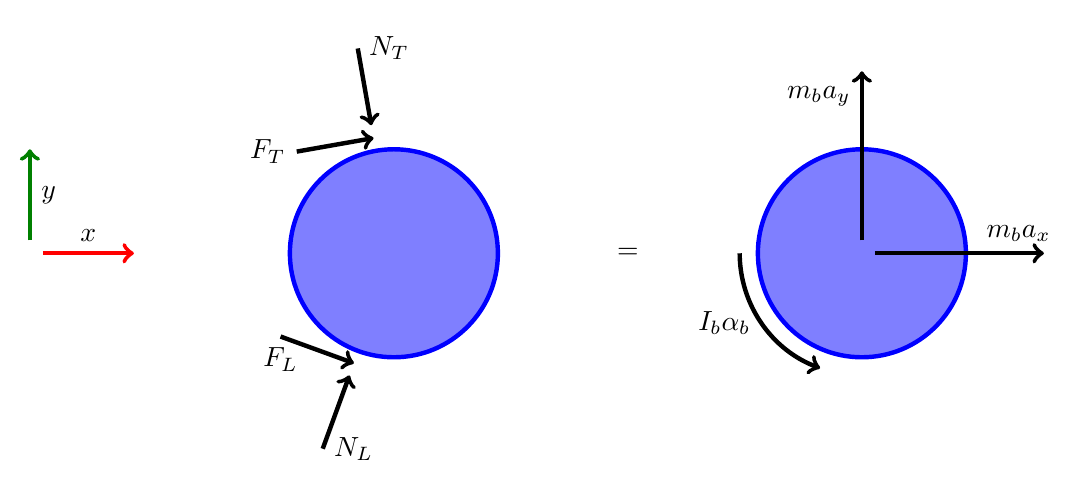
\begin{tikzpicture}[x=1.3in, y=1.3in]
	\draw[red, ultra thick, ->, shift={(-1.4,0)}] (0.05,0) -- (0.4,0) node[black,pos=0.5,above]{$x$};
	\draw[Green, ultra thick, ->, shift={(-1.4,0)}] (0,0.05) -- (0,0.4) node[black,pos=0.5,right]{$y$};
	\fill[Blue, ultra thick, opacity=0.5] (0,0) circle(0.4);
	\draw[Blue, ultra thick] (0,0) circle(0.4);
	\draw[Black, ultra thick, ->, rotate=-110] (.8,0) -- (0.5,0) node[pos=0, right]{$N_L$};
	\draw[Black, ultra thick, ->, rotate=-80] (-.8,0) -- (-0.5,0) node[pos=0, right]{$N_T$};
	\draw[Black, ultra thick, ->, rotate=-110] (0.45,-0.3) -- (0.45,0) node[pos=0, below]{$F_L$};
	\draw[Black, ultra thick, ->, rotate=-80] (-0.45,-0.3) -- (-0.45,0) node[pos=0, left]{$F_T$};

	\node[black] at (0.9,0) {=} ;

	\fill[Blue, ultra thick, opacity=0.5] (1.8,0) circle(0.4);
	\draw[Blue, ultra thick] (1.8,0) circle(0.4);

	\draw[Black, ultra thick, ->, shift={(1.8,0)}] (0,0.05) -- (0,0.7) node[pos=0.85, left]{$m_b a_y$};
	\draw[Black, ultra thick, ->, shift={(1.8,0)}] (0.05,0) -- (0.7,0) node[pos=0.85, above]{$m_b a_x$};
	\draw[Black, ultra thick, ->, shift={(1.8,0)}] (-0.47,0) arc (180:250:0.47) node[pos=0.5, left]{$I_b \alpha_b$};
	\end{tikzpicture}
	\caption{Free-Body and Kinetic Diagrams for Ball}
\end{figure}

\begin{align}
	F_T cos \psi + F_L cos \theta + N_T sin \psi + N_L sin \theta &= m_b a_x \\
	F_T sin \psi - F_L sin \theta - N_T cos \psi + N_L cos \theta &= m_b a_y \\
	F_L R_L - F_T R_T &= I_b \alpha_b
\end{align}

We will assume negligible vertical acceleration, so $a_y = 0$. We can then solve and find

\begin{align}
	a_x = \frac{F_T cos \psi + F_L cos \theta + N_T sin \psi + N_L sin \theta}{m_b} \\
	\alpha_b = \frac{F_L R_L - F_T R_T}{I_b}
\end{align}

As for the flywheel, there are two cases: the flywheels are separately powered and not linked, and the flywheels are centrally powered and linked. The indepdendent case is the same as that of the hooded pitcher, that is to say,
\begin{align}
	\alpha_{T,free}	&= - F_T \frac{d_T}{2 I_T} \\
	\alpha_{L,free}	&= - F_L \frac{d_L}{2 I_L}
\end{align}

In the linked case, a torque constrains the two wheels.

\begin{figure}[H]
	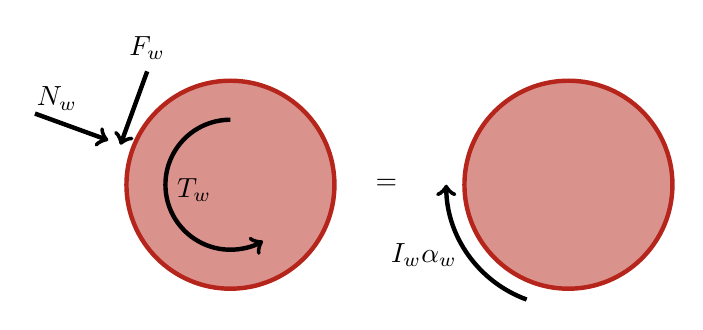
\begin{tikzpicture}[x=1.3in, y=1.3in]
	\fill[BrickRed, ultra thick, opacity=0.5] (0,0) circle(0.4);
	\draw[BrickRed, ultra thick] (0,0) circle(0.4);
	\draw[Black, ultra thick, ->, rotate=-20] (-.8,0) -- (-0.5,0) node[pos=0.3, above]{$N_w$};
	\draw[Black, ultra thick, ->, rotate=-20] (-0.45,0.3) -- (-0.45,0) node[pos=0, above]{$F_w$};
	\draw[Black, ultra thick, ->] (0,0.25) arc (90:300:0.25) node[pos=0.45, right]{$T_w$};

	\node[black] at (0.6,0) {=} ;

	\fill[BrickRed, ultra thick, opacity=0.5] (1.3,0) circle(0.4);
	\draw[BrickRed, ultra thick] (1.3,0) circle(0.4);
	\draw[Black, ultra thick, <-, shift={(1.3,0)}] (-0.47,0) arc (180:250:0.47) node[pos=0.5, left]{$I_w \alpha_w$};
\end{tikzpicture}
\caption{Free-Body and Kinetic Diagrams for Wheel}
\end{figure}

This leads to the torque balance

\begin{align}
	- N_w \frac{d_w}{2} - T_w = I_w \alpha_w \nonumber \\
	- F_T \frac{d_T}{2} - T_T = I_T \alpha_T \\
	- F_B \frac{d_B}{2} - T_B = I_B \alpha_B
\end{align}

The two wheels are coupled by a gear reduction $G$.

\begin{align}
	\alpha_L = \alpha_T * G \\
	- T_L * G = T_T
\end{align}

Solving these four equations yields

\begin{align}
	\alpha_{L,coupled} = \frac{- F_T \frac{d_T}{2 G} - F_L \frac{d_L}{2}}{I_L + I_T / G^2} \\
	\alpha_{T,coupled} = \alpha_L / G = \frac{- F_T \frac{d_T}{2 G} - F_L \frac{d_L}{2}}{G I_L + I_T / G} 
\end{align}

The ball can, again, be modeled as a spring.

\begin{figure}[H]
	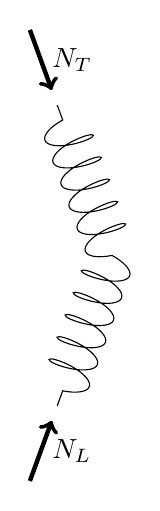
\begin{tikzpicture}[x=0.8in, y=0.8in]
	\draw[decoration={aspect=0.3, segment length=3mm, amplitude=3mm,coil},decorate, rotate=-20] (0,0) -- (0,-1);
	\draw[decoration={aspect=0.3, segment length=3mm, amplitude=3mm,coil},decorate, rotate=+20] (0,0) -- (0,+1);
	\draw[->, ultra thick, rotate=-20] (0,-1.5) -- (0,-1.1) node[pos=0.5, right]{$N_L$};
	\draw[->, ultra thick, rotate=+20] (0,+1.5) -- (0,+1.1) node[pos=0.5, right]{$N_T$};
	%\draw[->, ultra thick] (0,0) -- (-0.9,0) node[pos=.8, above]{$m_b a_{b,x}$};
	%\draw[->, ultra thick] (0,0) -- (0,-0.5) node[pos=.6, right]{$m_b a_{b,y}$};
	\end{tikzpicture}
	\caption{2-D spring model for ball}
\end{figure}

% Uh oh. This has rammifications

The friction model that follows is the same idea as that of the hooded pitcher, though it contains many more terms.

When the lower wheel grips:
\begin{align}
	v_{L,surf} = v_{b,bottom} \nonumber \\
	a_{L,surf} = a_{b,bottom} \nonumber \\
	\alpha_{L} \frac{d_L}{2} = a_{b} cos \theta + \alpha_{b} R_L \\
\end{align}

When the top wheel grips:
\begin{align}
	v_{T,surf} = v_{b,top} \nonumber \\
	a_{T,surf} = a_{b,top} \nonumber \\
	\alpha_{T} \frac{d_T}{2} = a_{b} cos \psi - \alpha_{b} R_T \\
\end{align}

First let's handle the simpler case of free, uncoupled wheels. For the lower side, we need to find $F_L$.
\begin{align}
	- F_L \frac{d_L}{2 I_L} \frac{d_L}{2} = (\frac{F_T cos \psi + F_L cos \theta + N_T sin \psi + N_L sin \theta}{m_b}) cos \theta + \frac{F_L R_L - F_T R_T}{I_b} R_L \\
	(\frac{N_T sin \psi + N_L sin \theta}{m_b}) cos \theta + F_T \frac{R_T}{I_b} R_L - \frac{F_T}{m_b} cos \psi cos \theta - F_L \frac{d_L}{2 I_L} \frac{d_L}{2} - \frac{F_L}{m_b} cos^2 \theta - F_L \frac{R_L^2}{I_b} = 0\\
	\textit{recognizing that this can be written in the form of } A + B F_T + C F_L = 0 \\
	A = (N_T sin \psi + N_L sin \theta) \frac{cos \theta}{m_b} \\
	B = \frac{R_T R_L}{I_b} - \frac{cos \psi cos \theta}{m_b} \\
	C = - \frac{d_L^2}{4 I_L} - \frac{cos^2 \theta}{m_b} - \frac{R_L^2}{I_b} \\
	F_{L,\ bottom\ gripped,\ free\ wheels} = \frac{A + B F_T}{- C}
\end{align}

For the top side, we need $F_T$.
\begin{align}
	- F_T \frac{d_T}{2 I_T} \frac{d_T}{2} = (\frac{F_T cos \psi + F_L cos \theta + N_T sin \psi + N_L sin \theta}{m_b}) cos \psi - \frac{F_L R_L - F_T R_T}{I_b} R_T \\
	(\frac{N_T sin \psi + N_L sin \theta}{m_b}) cos \psi - F_T \frac{R_T}{I_b} R_T - \frac{F_T}{m_b} cos^2 \psi - F_T \frac{d_T}{2 I_T} \frac{d_T}{2} + \frac{F_L}{m_b} cos \theta cos \psi - F_L \frac{R_L R_T}{I_b} = 0\\
	\textit{recognizing that this can be written in the form of } D + E F_L + F F_T = 0 \\
	D = (N_T sin \psi + N_L sin \theta) \frac{cos \psi}{m_b} \\
	E = \frac{R_L R_T}{I_b} - \frac{cos \theta cos \psi}{m_b} \\
	F = - \frac{d_T^2}{4 I_T} - \frac{cos^2 \psi}{m_b} - \frac{R_T^2}{I_b} \\
	F_{T,\ top\ gripped,\ free\ wheels} = \frac{D + E F_L}{- F}
\end{align}

The same analysis is repeated for the coupled flywheel case. When the lower wheel grips, we need to find $F_L$.
\begin{align}
	\frac{- F_T \frac{d_T}{2 G} - F_L \frac{d_L}{2}}{I_L + I_T / G^2} \frac{d_L}{2} = \nonumber \\
	(\frac{F_T cos \psi + F_L cos \theta + N_T sin \psi + N_L sin \theta}{m_b}) cos \theta + \frac{F_L R_L - F_T R_T}{I_b} R_L \\
	(\frac{N_T sin \psi + N_L sin \theta}{m_b}) cos \theta + F_T \frac{R_T}{I_b} R_L - \frac{F_T}{m_b} cos \psi cos \theta - F_T \frac{\frac{d_T}{2 G}}{I_L + I_T / G^2} \frac{d_L}{2} \nonumber \\
	- F_L \frac{\frac{d_L}{2}}{I_L + I_T / G^2} \frac{d_L}{2} - \frac{F_L}{m_b} cos^2 \theta - F_L \frac{R_L^2}{I_b} = 0\\
	\textit{recognizing that this can be written in the form of } A + B F_T + C F_L = 0 \\
	A = (N_T sin \psi + N_L sin \theta) \frac{cos \theta}{m_b} \\
	B = \frac{R_T R_L}{I_b} - \frac{cos \psi cos \theta}{m_b} - \frac{\frac{d_T d_L}{4 G}}{I_L + I_T / G^2} \\
	C = - \frac{\frac{d_L^2}{4}}{I_L + I_T / G^2} - \frac{cos^2 \theta}{m_b} - \frac{R_L^2}{I_b} \\
	F_{L,\ bottom\ gripped,\ free\ wheels} = \frac{A + B F_T}{- C}
\end{align}

For the top side, we need $F_T$.
\begin{align}
	\frac{- F_T \frac{d_T}{2 G} - F_L \frac{d_L}{2}}{G I_L + I_T / G} \frac{d_T}{2} = \nonumber \\
	(\frac{F_T cos \psi + F_L cos \theta + N_T sin \psi + N_L sin \theta}{m_b}) cos \psi - \frac{F_L R_L - F_T R_T}{I_b} R_T \\
	(\frac{N_T sin \psi + N_L sin \theta}{m_b}) cos \psi - F_T \frac{R_T}{I_b} R_T - \frac{F_T}{m_b} cos^2 \psi - F_T \frac{\frac{d_T}{2 G}}{G I_L + I_T / G} \frac{d_T}{2} \nonumber \\
	- F_L \frac{\frac{d_L}{2}}{G I_L + I_T / G} \frac{d_T}{2} - \frac{F_L}{m_b} cos \theta cos \psi + F_L \frac{R_L R_T}{I_b} = 0 \\
	\textit{recognizing that this can be written in the form of } D + E F_L + F F_T = 0 \\
	D = (N_T sin \psi + N_L sin \theta) \frac{cos \psi}{m_b} \\
	E = \frac{R_L R_T}{I_b} - \frac{\frac{d_L d_T}{4}}{G I_L + I_T / G} - \frac{cos \theta cos \psi}{m_b} \\
	F = - \frac{\frac{d_T^2}{4 G}}{G I_L + I_T / G} - \frac{cos^2 \psi}{m_b} - \frac{R_T^2}{I_b} \\
	F_{T,\ top\ gripped,\ free\ wheels} = \frac{D + E F_L}{- F}
\end{align}

For the case of both being gripped, we simply solve simultaneously.
\begin{align}
	A + B F_T + C F_L = 0 \text{ and } D + E F_L + F F_T = 0 \nonumber \\
	F_{L,\ both\ gripped} = \frac{A F-B D}{B E-C F} \\
	F_{T,\ both\ gripped} = \frac{C D-A E}{B E-C F}
\end{align}

State is determined as

\begin{align}
	\textit{top attached when } \omega_{T} \frac{d_T}{2} \leq v_{b} - \omega_{b} R_T \\
	\textit{lower attached when } \omega_{L} \frac{d_L}{2} \leq v_{b} + \omega_{b} R_L .
\end{align}

	All that's left is to set up the state equations and initial conditions.

	\begin{align}
		\frac{d}{dt} \omega_b &= \alpha_b \\
		\frac{d}{dt} v_b &= a_b \\
		\frac{d}{dt} x &= v_b \\
		\frac{d}{dt} \omega_T &= \alpha_T \\
		\frac{d}{dt} \omega_L &= \alpha_L \\
		v_b(0) &= 0 \\
		x(0) &= 0 \\
		\omega_T(0) &= \omega_{T,0} \\
		\omega_L(0) &= \omega_{L,0} \\
		\textit{when} \ x > x_end \ \textit{terminate}
	\end{align}

\section*{Hybrid Pitchers}
An interesting design proliferated during the FRC 2020 season, consisting of a hooded pitcher with an extra set of 'afterburner' wheels where the hood would terminate. This could be modeled fairly easily (I simply haven't gotten to it yet). I may transfer the calculator into a single one consisting of only the hybrid pitcher, as hooded and dual-wheel pitchers could be considered just special cases.

%\section*{Evaluation and Comparison to Empirical Data}

\end{document}